
\begin{enumerate}
    \item A small particle of mass \( m \) moving inside a heavy, hollow and straight tube along the tube axis undergoes elastic collision at two ends. The tube has no friction and it is closed at one end by a flat surface while the other end is fitted with a heavy movable flat piston as shown in figure. When the distance of the piston from closed end is \( L = L_0 \), the particle speed is \( v = v_0 \). The piston is moved inward at a very low speed \( V \) such that \( V \ll \frac{v_0}{L} \), where \( dL \) is the infinitesimal displacement of the piston. Which of the following statement(s) is/are correct?
        \begin{tasks}(2)
        	\task The rate at which the particle strikes the piston is \( v/L \)
        	\task After each collision with the piston, the particle speed increases by \(2V\)
        	\task If the piston moves inward by \(dL\), the particle speed increases by \(2v_0 \frac{dL}{L}\)
        	\task The particle’s kinetic energy increases by a factor of 4 when the piston is moved inward from \(L_0\) to \(\frac{1}{2}L_0\)
        \end{tasks}
    \item[\null] \textit{Diagram:}
        \begin{center}
            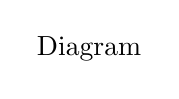
\begin{tikzpicture}
                \node at (0,0) {Diagram};
            \end{tikzpicture}
        \end{center}
\end{enumerate}
